\epigraph{The difference between ideas and reality is like the
difference between philosophy and engineering. The work to transform one into
the other is scientific research}{{\itshape V-Research}}

Several standards mandates a secure-by-design approach in which 
cybersecurity shall be considered at the very early stages of the 
design process. For example,
\begin{enumerate}[noitemsep]
	\item DO-326A -- ``Airworthiness Security Process Specification''
		requires a cybersecurity risk assessment of the design and is
		the ``are the only Acceptable Means of Compliance (AMC) by FAA
		\& EASA for aviation cyber-security airworthiness certification,
		as of 2019'' as pointed out by SAE in \autocite{SAE2019DO326A}.
	\item NIST 800-82 \autocite{Stouffer2011guide} -- ``guide to Industrial
		Control System (ICS) Security''
	\item J3061:2016-1 \autocite{SAE2016J3061} -- ``Cybersecurity Guidebook
		for Cyber-Physical Vehicle Systems'' defines ``set of
		high-level guiding principles for Cybersecurity as it relates
		to cyber-physical vehicle systems'' and states that
		``incorporate Cybersecurity into cyber-physical vehicle systems
		from concept phase through production, operation, service, and
		decommissioning''
\end{enumerate}
Companies which develop CPS (e.g. aerospace systems or elevator systems), must adhere
to strict regulations and quality assurances processes. Introducing tools and procedures 
in their processes requires a detailed and justified overview on how those
tools and procedures can be used. In Figure~\ref{fig:spdl}, we provide an overview
of a process that consider cybersecurity in the specification, design, and implementation
stages. The overall process start with the specification of the architectural (both physical
and functional) requirements from which the Weaknesses are automatically identified.
Based on the Assets, architectures, and the Weaknesses the cybersecurity risk is
calculated based on the $\abftheory$-theory. An iterative process between 
the user (e.g. the engineer) and the \secramod{} module of the \abftool{} allows the user to move to the design phase
when the risk level is considered acceptable. The design phase starts by automatically mapping
the Weaknesses into Vulnerabilities which are, in turn, fed into the \designverifmod{}
module along with the final specification. The Module returns a list of Vulnerabilities and
potential Mitigations. The user then procees in implementing the CPS and the SW/HW choices
can be tested by the \atgmod. \fix{mr}{While we have described the overall view, from
specification to implementation, in this text we only consider the process from specification to design.}

\begin{figure}[t]
	\centering
	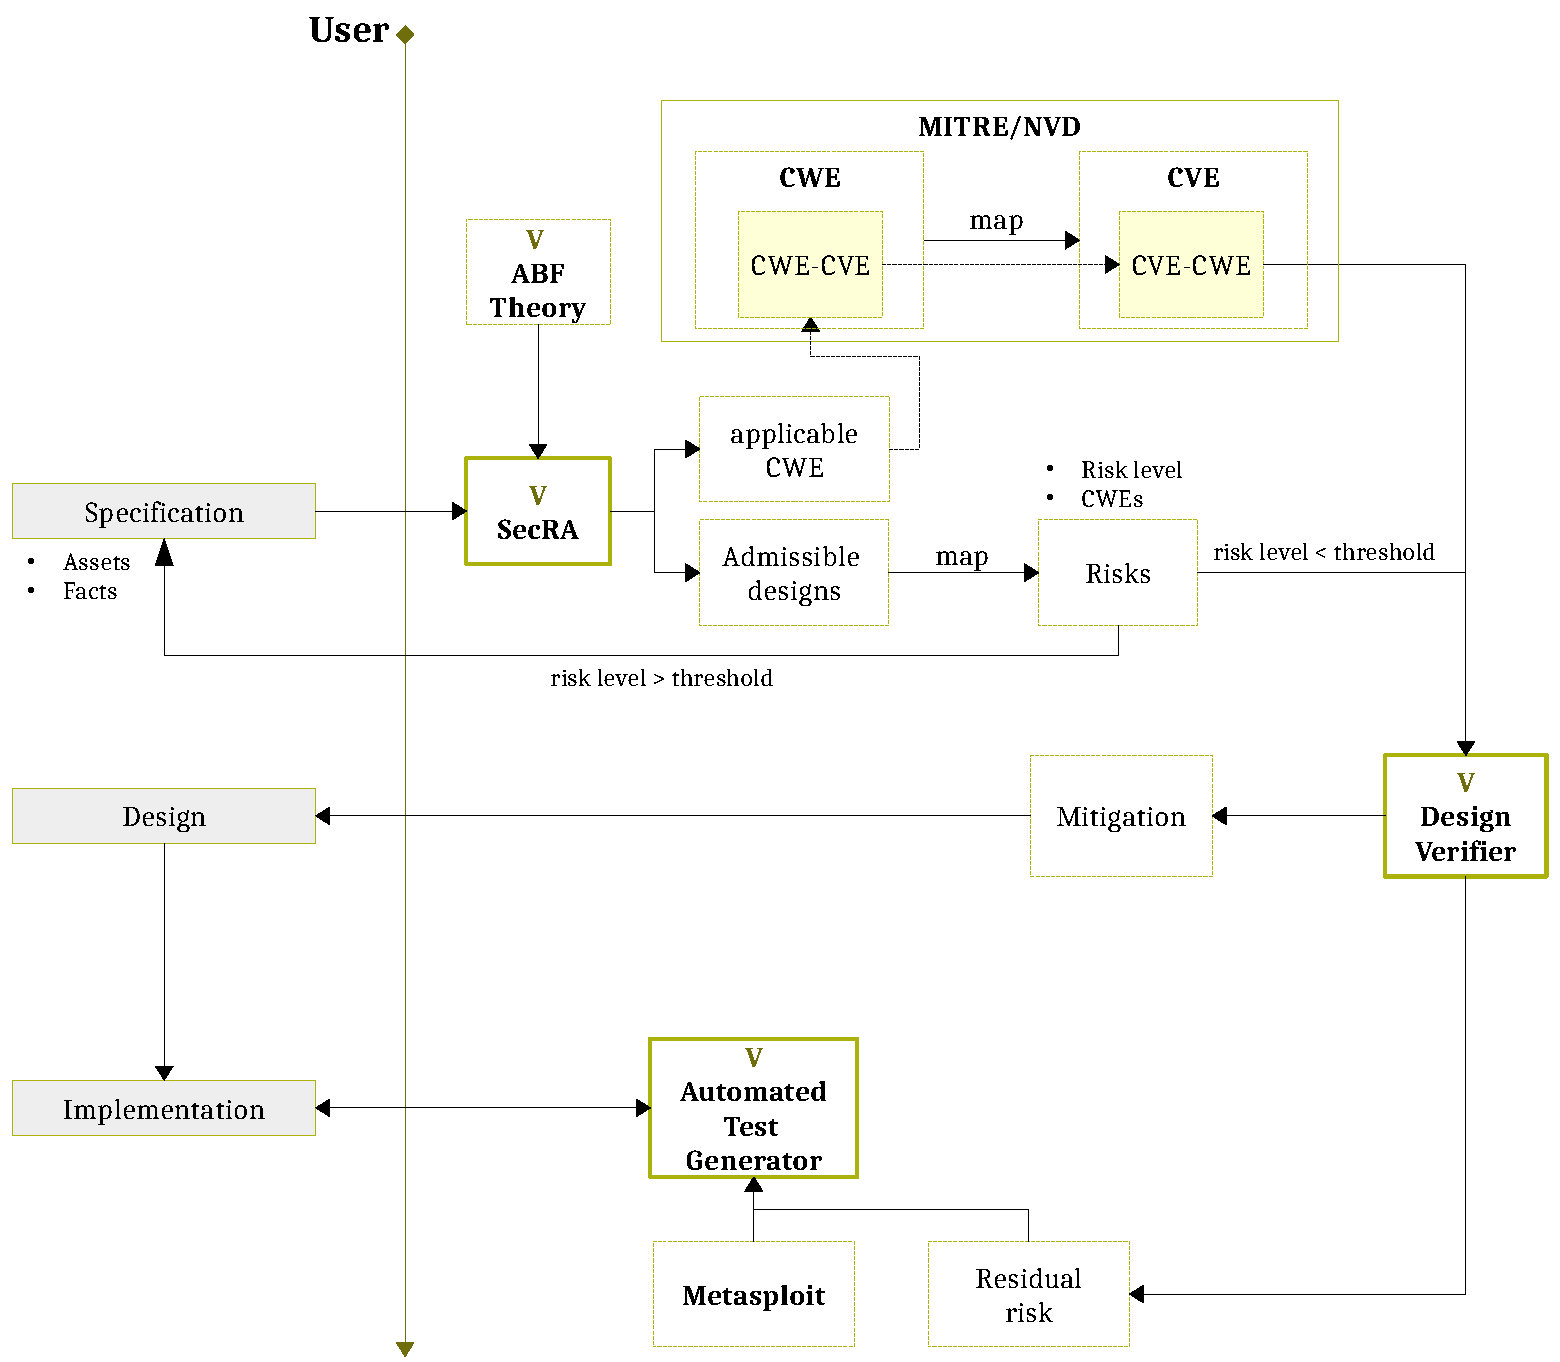
\includegraphics[width=\textwidth]{spdl.pdf}
	\caption{Secure-by-design System Development Life-cycle}
	\label{fig:spdl}
\end{figure}

In order to explain in details the SPDL, we use the following running example.
\begin{example}
	As depicted in Figure~\ref{fig:usecase}, the use case of the running example
	(a small part of a subprocess of the SwAT testbed \autocite{Mathur2016swat}), shows
	\begin{itemize}[noitemsep]
		\item a tank that is filled with raw water coming from the inlet pipe 
		\item a motorized valve (a valve with an actuator) such that:
			\begin{itemize}
				\item if opened, allows the raw water to flow into the tank
				\item if closed, stops the raw water to flow into the tank
			\end{itemize}
		\item a sensor that reads the meters of raw water in the tank
		\item a PLC controller, connected to the sensor and the
			actuator, that receives the readings from the sensor
			and regulates the quantity of water in the tank by
			communicating a change in the state of the actuator
			based on the following logic
			\begin{itemize}
				\item if the readings from the sensor reports a
					water level in the tank above (or
					equal) to 10m, the actuator shall close
					the valve
				\item if the readings are below 10m the actuator
					shall open the valve.
			\end{itemize}
	\end{itemize}

\begin{figure}[t]
	\centering
	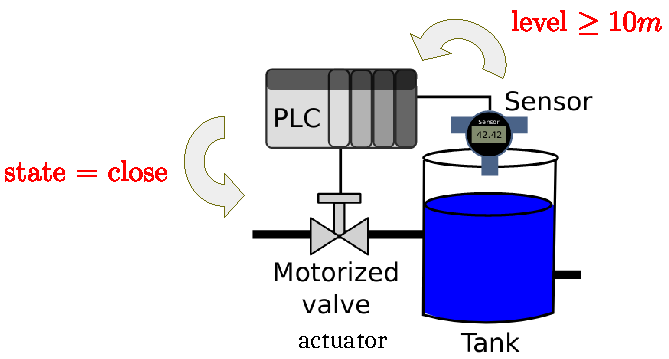
\includegraphics[width=.55\textwidth]{usecase.pdf}
	\caption{Use Case -- Running Example}
	\label{fig:usecase}
\end{figure}
\end{example}

\subsection{Specification -- Elicitation of Security Requirements}\label{sec:properties}
\begin{figure}[t]
	\centering
	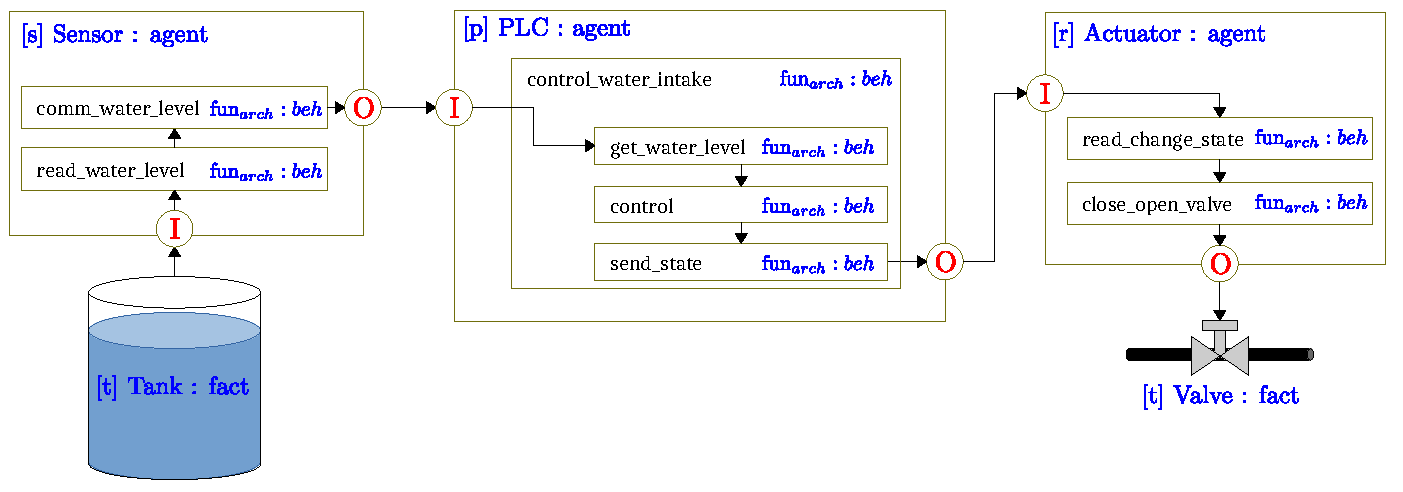
\includegraphics[width=\textwidth]{spec.pdf}
	\caption{Specification -- Running Example}
	\label{fig:spec}
\end{figure}
The first step of the SPDL is the definition of the requirements and then, for
the purpose of this paper, of (i) security requirements, (ii) architectural
(physical and functional) requirements.  Our focus in mainly on security
requirements but they are necessarily intertwined with the architectural
requirements, as we will show afterwards in this section.  A complete study on
how to properly define the architectural requirements is outside the scope of
this paper so we propose a method that is convenient for the purpose of our
assessment.

\paragraph{System Requirements}
In our running example, there is a system (a CPS) composed by $5$ main
subsystem which we consider atomic (i.e. not themself composed by subsystems)
and then agents: the tank, the sensor, the controller, the actuator, and the
motorized valve (valve from now on).  The whole specification (which we now
describe) of the physical and functional architecture is depicted in
Figure~\ref{fig:spec}.  In the use case, the communication flow is as follows:
\begin{enumerate}
	\item the sensor reads the level of water in the tank ($\text{tank}\rightarrow \text{sensor}$) \footnote{this communication depends on the technology in use for the readings. We assume a unidirectional communication without loss of generality}
	\item the sensor communicates the readings to the controller ($\text{sensor}\rightarrow \text{controller}$)
	\item the controller calculates the state of the valve and communicates it to the actuator ($\text{controller}\rightarrow \text{actuator}$)
	\item the actuator translates (digital to analog) the state received and communicates\footnote{we do not distinguish, for the sake of simplicity between different types of channels and assume that communicating to the valve produces the expected change of physical state} it to the valve
\end{enumerate}
Each agent has an input or output port from which it communicates with other
agents.  It is also composed by the functional blocks that defines its
functional architecture and physical boundaries that defines its physical
architecture, as detailed in Appendix~\ref{app:requirements}.

\begin{figure}[t]
	\centering
	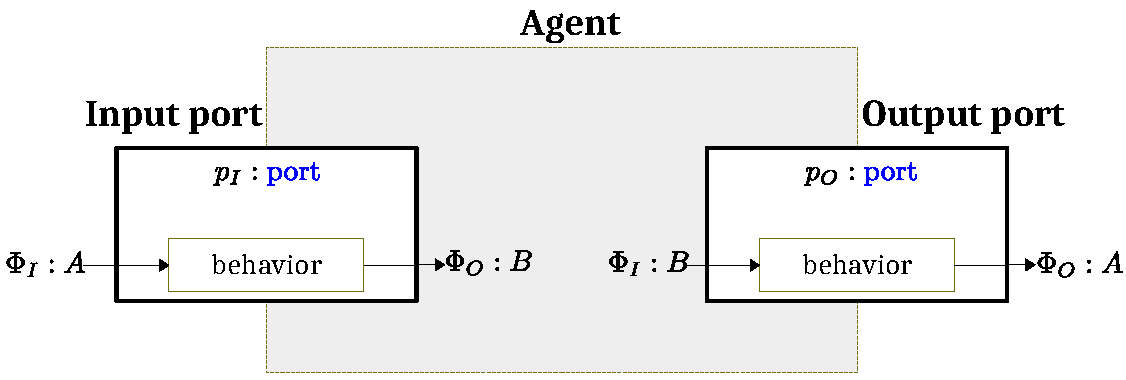
\includegraphics[width=.9\textwidth]{IOports.pdf}
	\caption{Input and Output Port of an agent}
	\label{fig:ioports}
\end{figure}

\begin{figure}[t]
	\centering
	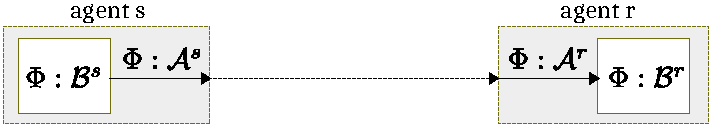
\includegraphics[width=.9\textwidth]{channel.pdf}
	\caption{Communication over a Mono-directional Channel}
	\label{fig:channel}
\end{figure}

While \emph{agents} and \emph{communication} between agents are described and
defined in Section~\ref{sec:theory}, the concepts of \emph{port} (depicted in
Figure~\ref{fig:ioports}), \emph{channel} (depicted in
Figure~\ref{fig:channel}), \emph{functional and physical architecture}, and
\emph{functional block} have not yet been defined with respect to the
$\abftheory$-theory.  Informally, a channel\footnote{for now, we rely on the
intuitive notion of channel as ``something'' that transfers information as
Assertions between output and input port, i.e. mono-directional} identifies the
place where the communication takes place.  In this work, we only consider
mono-directional channels and communication but the extension to bi-directional
channel can be considered as the union of two unidirectional channels. A
mono-directional channel is defined by the assertions sent or received (over
the channel). 

\subsubsection{Input and Output Ports}
Since the $\abftheory$-theory is a theory of agents, we consider ports as agents that
allows the exchange of information between a channel and another
agent.  However, a port must be considered as a special type of agent to avoid
an \emph{infinite regress} in which a port needs a port to transfer information
between the outside of the port to the inside of itself.

\begin{definition}{\bf Input or Output Port --}\label{def:port} 
	Ports are agents with the following predefined behavior: an input-port changes
	the type of information from assertion from a sender $s$ to an agent $a$,
	$\rassert{s}{a}$ to belief of the agent $a$ ($\beliefRegion_a$) while an
	output-port from belief to assertion; forwarding information from the outside
	of an agent's boundary to the inside (input-port) or vice versa (output-port). 
\end{definition}
The \emph{quality of a port} is determined by the $\rcc$ relation between the 
assertions received or sent and the belief, i.e. $\Rcc{\assertionRegion_s}{\beliefRegion_a}$ for the input-port
or $\Rcc{\assertionRegion_r}{\beliefRegion_a}$. We only define secure input port but the
definition of a secure output port is symmetrical.

\begin{definition}{\bf Secure Input Port --}\label{def:secport}
	A secure input port ($s\secureport a$) allows information as incoming assertions to flow
	from a sender $s$ to the behavior of the recipient $a$ (agent).  If $p_I$ is a secure input port,
	$\world\models\varphi$, $\varphi\in\rassert{s}{a}$, and $a$
	has the only input port $p_I$, $\world'\models\beliefRegion_a$ and $\varphi\in\beliefRegion_a$ for any
	$\world\modalrelation\world'$.
\end{definition}

\paragraph{Port Weaknesses}
From this definition, it follows that there exist only the following \emph{six} types of weaknesses, generating six types of insecure port in RCC5 (the notation is reported for input-ports, i.e. on the lef-hand side of the arrow):
\begin{enumerate}[start=1, label={W\arabic*)}]
	\item \emph{replace port} ($s\dropport a$), where assertions reaches the port but do not pass the boundary of the agent (i.e. do not become belief of the agent)
	\item \emph{drop port} ($s\dropport a$), where assertions reaches the port but do not pass the boundary of the agent (i.e. do not become belief of the agent)
	\item \emph{insertion port} ($s\insertport a$), where some new information is believed by $a$ as incoming from the port but $s$ didn't send it
	\item \emph{injection port} ($s\injectionport a$), where information coming from $s$ is substituted with new information which becomes believed by $a$
	\item \emph{selective port}, where some information passes the port and part is either:
	\begin{enumerate}[start=1, label={W4.\arabic*)}]
		\item drop ($s\selectivedropport a$), 
		\item drop+insert ($s\selectiveinsertport a$), or
		%\item injection ($s\selectiveinjectionport a$)
\end{enumerate}
\end{enumerate}

\fixnote{mr}{this proof needs to be restructured as in slides v-research-demo}
\begin{proof}
An input port is, in the $\abftheory$-theory, defined secure as long as the relation
	between the two regions of input assertions $\assertionRegion$ and
	output beliefs $\beliefRegion$ are equal, i.e.
	$\eq{\assertionRegion}{\beliefRegion}$. Therefore, any other relation
	should result in a weakness (related to an insecurity flaw) of that
	input port.  Using RCC5, there exist exactly other $4$ different type
	of relations, one of which is the discrete-from (DR) relation, i.e.
	$\dr{\assertionRegion}{\beliefRegion}$. When two regions are related by
	the DR relations, they have no subregion in common. Lets
	define a function weight $|X|$ such as, for any region $X$, it
	represents the smallest possible cardinality of a (mereo)topological base for
	$X$; where a base is a collection of regions in a (mereo)topology such that
	every open region can be written as union of elements of that base. 
	We distinguish between Regions that contain Information and Regions that
	don't by writing the latter as $\emptyset$.
	\begin{enumerate}
		\item if $\eq{\assertionRegion}{\beliefRegion})$ then either $\assertionRegion=\beliefRegion=\emptyset$ (no communication) or $\assertionRegion=\beliefRegion\neq\emptyset$ (forward communication)
		\item if $\dr{\assertionRegion}{\beliefRegion})$ then $\assertionRegion=\emptyset\oplus\beliefRegion=\emptyset$ (we call \emph{insert} the former and \emph{full drop} the latter case), or $\assertionRegion\neq\emptyset\wedge\beliefRegion\neq\emptyset\wedge\assertionRegion\neq\beliefRegion$ which we call \emph{replace} (i.e. drop and insert)
		\item if $\pp{\assertionRegion}{\beliefRegion})$ then $\beliefRegion$ contains and extend $\assertionRegion$ which we call \emph{injection}
		\item if $\ppi{\assertionRegion}{\beliefRegion})$ then $\assertionRegion$ contains and extend $\beliefRegion$ which we call \emph{selective drop}
		\item if $\po{\assertionRegion}{\beliefRegion})$ then a part of the $\assertionRegion$ is contained in the $\beliefRegion$ which is a combination of \emph{selective drop and generation}
	\end{enumerate}

	%	If
	%	a communication occurred and resulted in
	%	$\dr{\assertionRegion}{\beliefRegion}$, there exist only two mutually
	%	exclusive options: either $|\assertionRegion|=|\beliefRegion|$ or
	%	$|\assertionRegion|\neq|\beliefRegion|$. 
	%	\begin{itemize}
	%		\item If $|\assertionRegion|\neq|\beliefRegion|$ (at the end of
	%			a communication through the input-port), the two
	%			regions have a different number of subregions, and,
	%			then, there exist only two mutually exclusive options: 
	%			\begin{itemize}
	%				\item either $|\assertionRegion|>|\beliefRegion|$, where one
	%					ore more Assertions didn't become Beliefs, which we
	%					call \emph{drop port} ($s\dropport a$) since its behavior drops and
	%					prevents incoming communications,
	%				\item or $|\assertionRegion|<|\beliefRegion|$, where there are
	%					one ore more Beliefs which have not been sent as
	%					input-Assertions, which we call \emph{insertion
	%					port} ($s\insertport a$) since its behavior generates new Beliefs
	%					unrelated to the incoming communication. 
	%			\end{itemize}
	%		\item If $|\assertionRegion|=|\beliefRegion|$, supposing an increasing monotonic entropy on the information (Assertions) exchanged, 
	%				there exist only two mutually exclusive options: 
	%			\begin{itemize}
	%				\item either information has been generated as Belief and transferred as Assertions, increasing the cardinality of both
	%					$\assertionRegion$ and $\beliefRegion$, i.e.
	%					$|\assertionRegion_{t^0}|>|\assertionRegion_{t^1}|$ and
	%					$|\beliefRegion_{t^0}|>|\beliefRegion_{t^1}|$ (where
	%					$t^0$ and $t^1$ represent time at the beginning of
	%					communication and right after, respectively); which
	%					means that Assertions have reached the port and new
	%					Beliefs have been generated by the port, but no
	%					correlation between the elements of the two regions exist. 
	%					We call this \emph{injection port} ($s\injectionport a$) since it has modified
	%					the information carried by the Assertions into new
	%					corresponding Beliefs.
	%				\item or $|\assertionRegion_{t^0}|=|\assertionRegion_{t^1}|$
	%					and $|\beliefRegion_{t^0}|=|\beliefRegion_{t^1}|$ but
	%					this implies that no communication occurred, while we
	%					assumed that a communication was taking place (absurd).
	%			\end{itemize}
	%\end{itemize}
	%In other words, $\dr{\assertionRegion}{\beliefRegion}\equiv\neg\overlaps{\assertionRegion}{\beliefRegion}\equiv\neg(\varphi\subseteq\assertionRegion\wedge\varphi\subseteq\beliefRegion)\equiv\varphi\not\subseteq\assertionRegion\vee\varphi\not\subseteq\beliefRegion$
	%Similarly, 
	%\begin{itemize}
	%	\item given that $\po{\assertionRegion}{\beliefRegion}$ is equivalent to
	%		$\dr{\assertionRegion}{\beliefRegion}$ except for the
	%		overlapping part (see Appendix~\ref{app:selectiveinjectionport}) in which case is
	%		$\eq{\assertionRegion}{\beliefRegion}$ (see
	%		\autocite{Santaca2016abf}),
	%		we call it a \emph{selective injection port} ($s\selectiveinjectionport a$); otherwise
	%	\item $\pp{\assertionRegion}{\beliefRegion}\equiv\assertionRegion\Leftarrow\beliefRegion$ and
	%		$\ppi{\assertionRegion}{\beliefRegion}\equiv\assertionRegion\Rightarrow\beliefRegion$ are subcases of
	%		$\eq{\assertionRegion}{\beliefRegion}\equiv\assertionRegion\Leftrightarrow\beliefRegion$, and then
	%	\begin{itemize}
	%		\item if $\pp{\assertionRegion}{\beliefRegion}$, we have that
	%			some Beliefs are not correlated to incoming Assertions
	%			and we call it \emph{selective insertion port} ($s\selectiveinsertport a$),
	%		\item if $\ppi{\assertionRegion}{\beliefRegion}$ we have that
	%			some incoming Assertions are not correlated to Belief 
	%			and we call it \emph{selective drop port} ($s\selectivedropport a$)
	%	\end{itemize}
	%\end{itemize}
\end{proof}

\subsubsection{Communication Channels}
We start by considering the difference between a (communication)
mono-directional channel (channel from now on) and an agent, as we did for the
ports, since the $\abftheory$-theory is a theory of agents.  In fact, if a channel
were considered an agent (channel-agent) then the question would be how an
agent would transfer its Assertions to the channel-agent. If the channel
between the agent and the channel-agent is again an agent, we would generate an
\emph{infinite regress}. Therefore, we do allow channel-agents but we assume a
finite depth (of detail) for a channel, where there exists a bottom-channel
which is not an agent. For now, we do not constrain a channel-agent in any way
so there is no difference between a channel agent and agent. Therefore, for the
sake of simplicity, we consider, in this text, channels to be bottom-channels,
defined as agents with the pre-defined behavior (i.e. defined in a axiomatic
way) of forwarding any input-assertion as output-assertion, without modifying it\footnote{Nothing
prevents us from introducing additional constraints to the channel as storing
Assertions that are transferred over the channel, or filter out some
input-assertions.}. A port is, in fact, syntactic sugar to express the 
relation between Assertions and Beliefs.

\begin{definition}{\bf Secure Mono-directional Channel (bottom-channel) --}\label{def:monochannel}
	A mono-directional channel between the two agents ($s \rightarrow r$) is defined as 
	an agent which behavior is (dogmatically) defined as: to forward any Assertion received from $s$ over an input-port, to  
	the output-port where $r$ is listening to.
\end{definition}
The \emph{quality of a mono-directional} channel is defined as the 
$\rcc$ relation between the Assertions made by the sender and the ones received by the receiver, i.e. $\Rcc{\assertionRegion_s}{\assertionRegion_r}$.

\paragraph{Channel Weaknesses}
Given that a mono-directional bottom-channel is assumed to be perfectly
forwarding any Assertion from its input-port to its output-port, there is no
insecure behavior but only the combination of the weaknesses of the input and
output port; therefore there exists $(7^2)-2=47$ theoretical configurations
($7^2$ because there are $6$ insecure types of port, plus $1$ secure type, on both input and oupput
side; and we exclude the configuration with $2$ secure types as input
and ouput, $-2$); where only 43 are possible.

\begin{enumerate}[start=6, label={W\arabic*)}]
	\item \emph{secure output port} and \emph{input drop port} ($s\sdcom r$), 
	\item \emph{secure output port} and \emph{input insertion port} ($s\sicom r$), 
	\item \emph{secure output port} and \emph{input injection port} ($s\sjcom r$), 
	\item \emph{secure output port} and \emph{input selective drop port} ($s\ssdcom r$), 
	\item \emph{secure output port} and \emph{input selective insertion port} ($s\ssicom r$), 
	\item \emph{secure output port} and \emph{input selective injection port} ($s\ssjcom r$), 

	\item \emph{output drop port} and \emph{input drop port} ($s\ddcom r$)
	\item \emph{output drop port} and \emph{input insertion port} ($s\dicom r$)
	\item \emph{output drop port} and \emph{input secure port} ($s\dscom r$)

	\item \emph{output insert port} and \emph{input drop port} ($s\idcom r$)
	\item \emph{output insert port} and \emph{input insert port} ($s\iicom r$)
	\item \emph{output insert port} and \emph{input injection port} ($s\ijcom r$)
	\item \emph{output insert port} and \emph{input selective drop port} ($s\isdcom r$)
	\item \emph{output insert port} and \emph{input selective insertion port} ($s\isicom r$)
	\item \emph{output insert port} and \emph{input selective injection port} ($s\isjcom r$)
	\item \emph{output insert port} and \emph{input secure port} ($s\iscom r$)

	\item \emph{output injection port} and \emph{input drop port} ($s\jdcom r$)
	\item \emph{output injection port} and \emph{input insertion port} ($s\jicom r$)
	\item \emph{output injection port} and \emph{input injection port} ($s\jjcom r$)
	\item \emph{output injection port} and \emph{input selective drop port} ($s\jsdcom r$)
	\item \emph{output injection port} and \emph{input selective insertion port} ($s\jsicom r$)
	\item \emph{output injection port} and \emph{input selective injection port} ($s\jsjcom r$)
	\item \emph{output injection port} and \emph{input secure port} ($s\jscom r$)

	\item \emph{output selective drop port} and \emph{input drop port} ($s\sddcom r$)
	\item \emph{output selective drop port} and \emph{input insertion port} ($s\sdicom r$)
	\item \emph{output selective drop port} and \emph{input injection port} ($s\sdjcom r$)
	\item \emph{output selective drop port} and \emph{input selective drop port} ($s\sdsdcom r$)
	\item \emph{output selective drop port} and \emph{input selective insertion port} ($s\sdsicom r$)
	\item \emph{output selective drop port} and \emph{input selective injection port} ($s\sdsjcom r$)
	\item \emph{output selective drop port} and \emph{input secure port} ($s\sdscom r$)

	\item \emph{output selective insertion port} and \emph{input drop port} ($s\sidcom r$)
	\item \emph{output selective insertion port} and \emph{input insertion port} ($s\siicom r$)
	\item \emph{output selective insertion port} and \emph{input injection port} ($s\sijcom r$)
	\item \emph{output selective insertion port} and \emph{input selective drop port} ($s\sisdcom r$)
	\item \emph{output selective insertion port} and \emph{input selective insertion port} ($s\sisicom r$)
	\item \emph{output selective insertion port} and \emph{input selective injection port} ($s\sisjcom r$)
	\item \emph{output selective insertion port} and \emph{input secure port} ($s\siscom r$)

	\item \emph{output selective injection port} and \emph{input drop port} ($s\sjdcom r$)
	\item \emph{output selective injection port} and \emph{input insertion port} ($s\sjicom r$)
	\item \emph{output selective injection port} and \emph{input injection port} ($s\sjjcom r$)
	\item \emph{output selective injection port} and \emph{input selective drop port} ($s\sjsdcom r$)
	\item \emph{output selective injection port} and \emph{input selective insertion port} ($s\sjsicom r$)
	\item \emph{output selective injection port} and \emph{input selective injection port} ($s\sjsjcom r$)
	\item \emph{output selective injection port} and \emph{input secure port}  ($s\sjcom r$)
\end{enumerate}
In Appendix~\ref{app:insecurecom}, we report the proof which is exhaustive on all
possible combinations. 

\paragraph{Ports and Channels -- Discussion} 
It is important to note that all the results of the application of the
$\abftheory$ to channels is the analysis of the relation
$\rcc{\assertionRegion_o}{\assertionRegion_i}$ leads to the same results of the
analysis of a pair one input and one output port (i.e.
$\rcc{\beliefRegion_1}{\assertionRegion_2}\wedge\rcc{\assertionRegion_2}{\beliefRegion_3}$
The same result can be obtained by analyzing the relation
between the outputs of a functional block and the inputs of
another functional block.
As depicted in Figure~\ref{fig:atom}, so far, we have considered Information
generated by a Port $P_I$ and then sent through a channel $C$ to another
(recipient) port $P_O$. In this scenario where Ports and then Channels are
atomic (otherwise raising infinite regress), we can only  consider the
relations between Ports and Channel; considering both input-port to channel and
channel to output-port. In fact, the Weaknesses of a channel are defined in terms
of the Weaknesses of Ports. We now introduce the concept of
functional architecture and its decomposition into functional blocks. 
Io order to define a functional block without encountering a infinitely recursive definition,
we must reach the same conclusions as for the Channel. Therefore, describing
the information as flowing over a channel or in a functional block is purely
syntactic sugar.

We can summarize these results by saying that the relations
between Assertions and Beliefs, Output Assertions of an Agent and 
Input Assertions of another Agent, or Output Beliefs of a 
Functional Block and Input Beliefs of another Block can \emph{only}
be affected by the following weaknesses: replace,
drop, injection, insertion, selective drop, and selective drop + insertion.
We can, then, propose the following security properties:
\begin{itemize}
	\item \emph{Order-preserving} -- it shall be known if Information is \emph{replaced}
	\item \emph{Availability} -- it shall be known if Information is \emph{dropped} or \emph{selectively dropped}
	\item \emph{Integrity} -- it shall be known if Information is \emph{injected}
	\item \emph{Authentication} -- it shall be known if Information is \emph{inserted}
\end{itemize}

\begin{figure}[t]
	\centering
	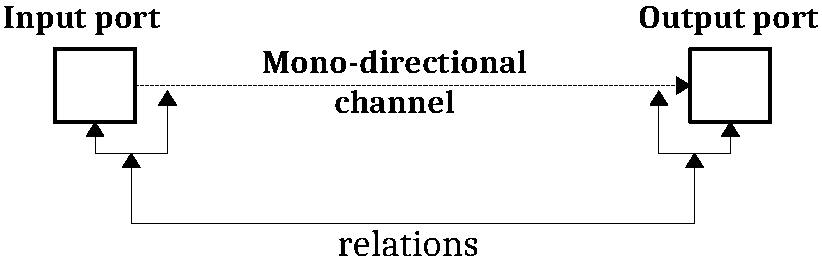
\includegraphics[width=.7\textwidth]{engineering_relations.pdf}
	\caption{Relations between Ports and Channel}
	\label{fig:atom}
\end{figure}

\subsubsection{Functional Block}
A Functional Architecture, as already described beforehand, takes Information as input-Beliefs
and transforms the Information into output-Beliefs. Those transformations 
occurs within the Functional Architecture, where Functional Blocks transforms Beliefs into 
other Beliefs. Similarly to channels, we could consider a Functional Block as a Functional Architecture
occurring in an infinite regress. Therefore, we consider Functional Blocks as 
executing an abstract undefined behavior, of which we only observe the
inputs and the resulting outputs (Beliefs).

\begin{definition}{\bf Functional Block and Architecture --}\label{def:funblock}
	A functional block of an agent 
	takes a region of input-Beliefs and outputs a region of output-Beliefs. 
	A functional architecture is an interconnected system of functional blocks.
\end{definition}
It is evident that the quality of a functional block cannot be determined
by the difference between its inputs and outputs (as we did for
ports and channels). The behavior of a functional block
cannot be determined in general; since any functional block will have 
its own purpose based on functional requirements. 
Therefore, while a port semantics is determined by the relation 
between Assertions and Beliefs, the semantics of a Functional Block 
is determined by the relation between Facts/Requirements and I/O Beliefs.

In other words, a functional block is a generic agent with no pre-defined general
behavior (while ports and channels have a pre-defined behavior).

\begin{itemize}
	\item $\po{\behaviorRegion}{\factRegion}$ the component has a Byzantine behavior where occasionally outputs the expected
	        output given the correct inputs. Not all the inputs are handled
	        properly, nor all the expected outputs are always generated
	        when correct inputs are given.
	\item $\pp{\behaviorRegion}{\factRegion}$ part of the expected outputs are not
	        generated in response to the correct
	        inputs
	\item $\ppi{\behaviorRegion}{\factRegion}$ the components
	        correctly performs the expected behavior when the correct
	        inputs are provided but is subject to input
	        injections
	\item $\dr{\behaviorRegion}{\factRegion}$ the component
		never performs the expected behavior (e.g. physical
		damage)
\end{itemize}

\paragraph{Requirements as Facts}
During the specification phase, for any agent, channel, port, functional block
and architecture, there may exist a factorial requirement (Fact) predicating over them.
In other words, any requirement is defined as a Fact since they must be true in
any design or implementation. As we stated in Section~\ref{sec:theory} and depicted in
Figure~\ref{fig:soundness}, Facts are strategic rules that defines how
the system shall behave (by specification), while reality may be shown to
be insecure.

\begin{figure}[t]
	\centering
	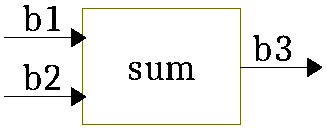
\includegraphics[width=0.3\textwidth]{sum.pdf}
	\caption{Example of a Functional Block}
	\label{fig:sum}
\end{figure}

As an example, consider a functional block that performs the summation of two
inputs, as in Figure~\ref{fig:sum}, defined by the requirement $r := b_3 = b_1
+ b_2$. The possible relations between the behavior of the functional block and
the requirements (i.e. $\Rcc{\behaviorRegion}{\factRegion}$ is determined by
the relations between the I/O Beliefs $sum(b_1,b_2)=b_3$ and the requirement
$sum(b_1,b_2)=b_1+b_2$, as follows.
\begin{itemize}
	\item $\eq{\beliefRegion}{\factRegion}=\eq{\beliefRegion_3}{\beliefRegion_1+\beliefRegion_2}$, 
		where $\beliefRegion_3$ represents the Region of all the
		outputs of the functional block $sum$ while the Region
		$\beliefRegion_1+\beliefRegion_2$ represents the expected
		outputs of an ideal implementation of the requirement $r$.
		Therefore, the functional block correctly implements the
		requirements.
	\item
		$\dr{\beliefRegion}{\factRegion}=\dr{\beliefRegion_3}{\beliefRegion_1+\beliefRegion_2}$,
		the function block never implements the requirements.
	\item
		$\pp{\beliefRegion}{\factRegion}=\pp{\beliefRegion_3}{\beliefRegion_1+\beliefRegion_2}$, there exist some inputs for which
		the output is incorrect.
	\item $\ppi{\beliefRegion}{\factRegion}=\ppi{\beliefRegion_3}{\beliefRegion_1+\beliefRegion_2}$, there exists some outputs that are not the result of the summation of the inputs but given the correct inputs the function always outputs correctly.
	\item
		$\po{\beliefRegion}{\factRegion}=\po{\beliefRegion_3}{\beliefRegion_1+\beliefRegion_2}$,
		the component has a Byzantine behavior where occasionally
		outputs the expected output given the correct inputs. Not all
		the inputs are handled properly, nor all the expected outputs
		are always generated when correct inputs are given.
\end{itemize}

\paragraph{Methodology}
We have now mapped the building blocks of our theory, namely Information,
Belief, Assertion, Behavior, and Fact. One may notice that the concept of
Knowledge hasn't been discussed in this section so far. Our argument is that
knowledge, as an epistemological concept cannot be defined due to several
implication that this would have (see, for example,
\autocite{Empiricus1990Pyrrhonism}). On the other hand, the factorial way in
which requirements are imposed may be true only in the specification, while not
necessarily true in the final implementation. While Knowledge may not be
apprehensible in general, we can define tests to see if Facts holds in a
design or implementation. What is of our interest is to guarantee security in a
system so we now correlate the potential behaviors with the standard (de-facto)
understanding of security; so that we can identify test that, at the end of the
engineering process, may not give Knowledge but, at last, tested Fact.

\subsubsection{Security Requirements} 
While standards such as IEC 62443-1-3 (the Industrial communication networks -
Network and system security -- Part 3-3: System security requirements and
security levels) defines requirements as ``confidentiality of information in
transit/at-rest'', we believe that, at specification level, a mapping
between the Infosec security concepts of the well-known CIA (Confidentiality,
Integrity, Availability) triad to the system components can be used to specify
a list of security requirements.

Infosec, or Information Security, defines the security risks related to
information as the CIA triad, which has been often criticized
(as we show afterwards) for being too general or non-adequate (e.g. by
adding authenticity which is often used as a building block for confidentiality
and integrity) to be effectively applied to the engineering of systems. Due to
this, many researchers and organization tried to improve the CIA triad.  The
evolutions/extensions of the CIA triad has been documented, e.g., in
\autocite{Samonas2014cia} and are summarized in Table~\ref{tab:ciaevolution}.

\begin{table}[h]
\centering
%\setlength{\tabcolsep}{3.5pt}
%\renewcommand{\arraystretch}{1}
\small
\begin{tabular}{rll} 
	{\bf Year} & {\bf Definition} & {\bf Legend}\\
	\hline
	1970s & infosec = CIA & Confidentiality, Integrity, Availability\\
	1980s & infosec += (Au, nR) & Authenticity and non-Repudiation\\
	1990s & infosec += CSpec & Correctness in Specification\\
	2000s & infosec += RITE & Responsibility, Integrity of people, Trust, Ethicality
\end{tabular}
\caption{Chronological progression of the CIA triad~\label{tab:ciaevolution}}
\end{table}


A representative example is the effort made by the OECD (Organisation for Economic
Co-operation and Development) in \autocite{OECD2013guidelines} to define
security guidelines for information system (1992) based on new principles such
as ``awareness, ethics, risk assessment'' and maintain those improving the document with
subsequent revisions 
(e.g.  following the multistakeholder expert consultation in 2013).
Other similar efforts focused on defining entirely new principles or extending
the CIA triad, such as \autocite{NISTSP800-160}. 
%What is of interest for our
%argument is that, to the best of our knowledge, all of the approaches that aim
%at improving the CIA triad are besed on motivations related to empirical evidences. On the contrary,
%We now define (in Section~\ref{sec:properties}) the CIA triad for an agent
%defined in the $\abftheory$-theory and we test if (i) other properties are
%allowed in the $\abftheory$-theory, and (ii) if and how the CIA triad can be
%detailed in the $\abftheory$-theory.
In \autocite{Anderson1972report,Samonas2014cia}, CIA are defined as follows.
\begin{itemize}
	\item \emph{Unauthorized information release}: an unauthorized person is able
		to read and take  advantage  of  information  stored  in  the
		computer.  This  category of concern  sometimes  extends  to
		``traffic  analysis,''  in  which  the intruder  only observes
		the  patterns  of  information  use.  From  those patterns,
		the  intruder can   infer   some   information   content.
		This category   also   includes   the unauthorized use of a
		proprietary program.  (Confidentiality or Secrecy) 
	\item \emph{Unauthorized  information  modification}:  an  unauthorized person
		is  able  to make changes in stored information -- a form  of
		sabotage.  It should be noted that in the case of this kind of
		violation, the intruder does not necessarily see the
		information he has changed.  (Integrity)
	\item \emph{Unauthorized  denial  of  use}:  an  intruder  can  prevent  an
		authorized  user  from referring to, or from modifying
		information, even though the intruder may not be able to refer
		to, neither modify the information themselves. (Availability)
\end{itemize}

We now want to generalize the CIA triad to agents and systems in the
$\abftheory$-theory (and not just Information). Given that we are currently
dealing with the step that moves from specification to design, we consider
architectural properties. For the sake of simplicity, we revert the order and
start from availability.

\paragraph{Availability and Integrity (Architecture Security)}
\begin{figure}[t]
	\centering
	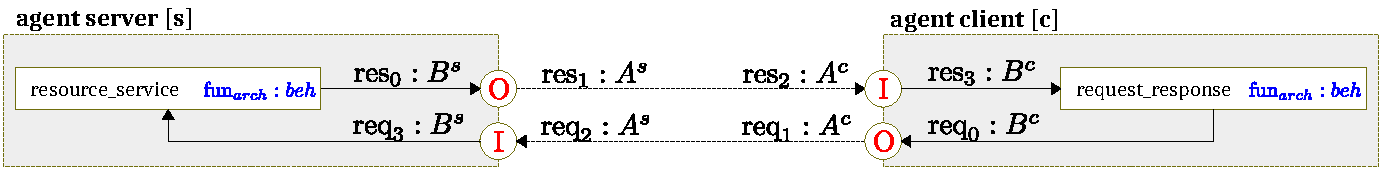
\includegraphics[width=\textwidth]{client-server.pdf}
	\caption{Client-Server paradigm in $\abftheory$-theory}
	\label{fig:client-server}
\end{figure}
Availability, again, is the denial of use of a resource. In the $\abftheory$-theory, 
in order to prevent a resource to be available, there
exists only (i.e. inclusively) the following cases
that we illustrate using a client-server paradigm (depicted in Figure~\ref{fig:client-server}).
\begin{enumerate}
	\item\label{case:srv1} The resource on the server cannot be found, so that it is
		possible for the client to contact the server and for the server
		to send a response back, but the output-port does not receive the
		necessary information. This may be due to a software error such
		that the functional architecture doesn't output a response, or
		a problem in the flow of information (i.e. the functional
		architecture doesn't receive the necessary information from
		other resources), or an hardware failure \&c. This can be formalized
		as an issue to be found in the relation between the beliefs produced by the functional
		architecture and the ones received by the output port, i.e.
		$\rcc(\behaviorRegion_s,\{\text{res}_0\})$ or 
		$\rcc(\beliefRegion_s,\{\text{res}_0\})$ 
	\item\label{case:srv2} The server hosting the resource is down, and then the server
		cannot output responses (i.e. insecure output port due to drop-related issue) or receive
		requests (insecure input port due to drop-related issue) or both.
	\item\label{case:srv3} The client cannot properly compute request (symmetric to Case~\ref{case:srv1})
	\item The client is down, symmetric to Case~\ref{case:srv2}
	\item The channel is down due to a drop related issue in one of the two channels 
\end{enumerate}
We shall, then, distinguish between two cases, as we mentioned beforehand:
agent (or system) and Information (which we call Infosec) availability. 
\begin{definition}{\bf Agent-Availability --}\label{def:agent-a}
when the property of availability is expressed over an agent or a system, the
	list of possible designs do not include those in which there exist:
	drop ports, or drop channels/functional-blocks.
\end{definition}
\begin{definition}{\bf Infosec-Availability --}\label{def:infosec-c}
when the property of availability is expressed
	over a formula, the list of possible designs that violates the
	availability property is reduced to the part of the system that
	does not influence that specific formula.
\end{definition}

In a similar way we can define integrity since this requirement may 
be expressed over an agent/system or a specific formula (i.e. element of a Region).

\begin{definition}{\bf Agent-Integrity --}\label{def:agent-a}
when the property of integrity is expressed over
	an agent or a system, the list of possible designs 
	do not include those in which there exist: insert or inject ports, 
	or insert or inject channels/functional-blocks. 
\end{definition}
\begin{definition}{\bf Infosec-Integrity --}\label{def:infosec-c}
when the property of integrity is expressed
	over a formula, the list of possible designs that violates the
	integrity property is reduced to the part of the system that
	influences that specific variable.
\end{definition}

While availability and integrity are architectural property, meaning that they
can be expressed over the behavior of a port or a channel (as constituent of
the physical or functional architecture), confidentiality is not.
Confidentiality states that an information shall not be understood and not that
the information shall not be retrieved. So, if a port leaks an entire message,
there is no confidentiality issue in general, unless that message was not
encrypted, in which case the confidentiality leakage is straightforward. 
On the other hand, if the
information is not provided or altered there is an availability or integrity
issue. A similar argument can be proposed for integrity sub-properties such as
authenticity or non-repudiation. No wonder why it is often stated that
availability and integrity are the first properties to be considered in CPS secure engineering
while confidentiality takes the first place when dealing with security
protocols. In fact, integrity is often assumed by pattern-matching (e.g. in
AVANTSSAR \autocite{Armando2012avantssar}) and availability is hardly ever considered in
protocol verification. The question is, can we express properties such as
confidentiality, authentication, or non-repudiation as architectural properties
in $\abftheory$-theory? Confidentiality is based on the concept 
of secrecy so we shall first start from describing what secrecy is and how it
can be used to guarantee confidentiality in a system.

\paragraph{Secrecy, Authenticity, and Key Agreement (Cryptographic Security)}\label{sec:encryption}
As Maurer puts it (\autocite{Maurer1999information}), there exist two types of
cryptographic security (i.e. scientific theories aiming at guaranteeing
security through the use of cryptographic functions): ``The security  of a
cryptographic system can rely either on the computational infeasibility of
breaking it (computational security), or on the theoretical impossibility of
breaking it, even using in infinite computing power (information-theoretic or
unconditional security)''. We are not currently interested in detailing the
difference between the two and we simplify it as follows. A
computationally-secure cryptographic function (usually called encryption
function) $E(\varphi)=e$ (where $\varphi$ is a plain-text and $e$ a
cipher-text) can be considered perfectly secure if a malicious agent that
obtains the result of the cryptographic function ($e$) has bounded
computational power, while unconditional secure cryptographic functions are
considered perfectly secure. In this context, security means that is is
impossible to calculate $\varphi$ from $e$, therefore impossible to compute
$D(e)=\varphi$.  As one can evince from \autocite{Shannon1948information}, the
commonality between the two types of cryptographic functions is that they both
rely on the assumption about the probabilistic behavior of the universe. They
do so, for the random (i.e. with high entropy
\autocite{Shannon1948information}) generation of the so called \emph{key}, a
piece of information, parametric to the cryptographic function, used to
guarantee the security. Therefore, we can assume that it is feasible for an
agent that knows $k$ to decrypt the cipher-text obtaining the clear-text (i.e. $D(k, E(k,\varphi))=\varphi$)
while it is impossible for any agent that has not the proper key. In this
case, the information is considered to be \emph{secret or confidential}.

\begin{definition}{\bf Infosec-Secrecy or Confidentiality --}\label{def:confidentiality}
	When an Assertion has been generated as an output by an
	agent, port, or functional block such that it is said (in a
	factorial way) to encrypt the input, that Assertion is considered
	confidential.
\end{definition}
The quality of the confidentiality of information (Assertions or Beliefs depending on 
the subsystem considered) is inversely proportional to the number of 
integrity issues of the subsystem.
We now discuss more in details what secrecy of Information is when 
dealing with functional blocks (Behavior) and Beliefs but a similar treatment can be done 
in the case of Channels and Assertions.

The quality of a Functional Block is determined by the relation between the
input-Beliefs formulas and the symmetric formulas in the Fact region
(equivalently for output-Beliefs).

\begin{definition}{\bf Secrecy of Functional Block and Architecture --}\label{def:secfun}
	Secrecy is preserved in a functional block if the input beliefs and output beliefs
	are in $EQ$ relation with the corresponding Facts mandated by the confidentiality/secrecy requirements.
	A functional architecture where all the secrecy-preserving functional blocks
	are in $EQ$ relation with the corresponding Facts
	is considered confidential/secrecy-preserving.
\end{definition}

\paragraph{Confidentiality Weaknesses}
In a functional block, there exists the following weaknesses in the functional
architecture, where $\beliefRegion_I$ and $\beliefRegion_O$ are input and
output Beliefs respectively, and $\factRegion_I$ and $\factRegion_O$ are
the corresponding Facts. 
\begin{itemize}
	\item $\eq{\beliefRegion_I}{\factRegion_I}$ and then only specified
		inputs can be fed to the functional block but:
	\begin{enumerate}[start=49, label={W\arabic*)}]
		\item\label{w:fb_eqdr} $\dr{\beliefRegion_O}{\factRegion_O}$, not all the specified
			outputs are produced. This may produce a secrecy issue if, for example,
			the functional block is responsible for generating an encryption key since
			if it is not produced the encryption of the Information may not be performed
		\item\label{w:fb_eqpo} $\po{\beliefRegion_O}{\factRegion_O}$, only some but not all of the specified
			outputs are produced along with some non-specified output are produced. This
			strightforwardly generates a secrecy when the functionality is 
			related to secrecy functional blocks since some outputs doesn't follow
			the requirements.
		\item $\pp{\beliefRegion_O}{\factRegion_O}$, not all the specified outputs are produced.
			This may pose a secrecy issue as in \ref{w:fb_eqdr}
		\item $\ppi{\beliefRegion_O}{\factRegion_O}$, not all the output have been specified.
			This may pose a secrecy issue as in \ref{w:fb_eqpo}
	\end{enumerate}
	\item $\po{\beliefRegion_I}{\factRegion_I}$, not all the specified inputs can be fed into the functional block
	\begin{enumerate}[start=53, label={W\arabic*)}]
		\item $\dr{\beliefRegion_O}{\factRegion_O}$
		\item $\po{\beliefRegion_O}{\factRegion_O}$
		\item $\pp{\beliefRegion_O}{\factRegion_O}$
		\item $\ppi{\beliefRegion_O}{\factRegion_O}$
		\item $\eq{\beliefRegion_O}{\factRegion_O}$ this case implies
			that somehow there is no input that generates an
			non-specified output but this is not because the inputs
			are secure 
	\end{enumerate}
	\item $\pp{\beliefRegion_I}{\factRegion_I}$, not all the specified
		inputs can be fed into the block
	\begin{enumerate}[start=58, label={W\arabic*)}]
		\item $\dr{\beliefRegion_O}{\factRegion_O}$
		\item $\po{\beliefRegion_O}{\factRegion_O}$
		\item $\pp{\beliefRegion_O}{\factRegion_O}$
		\item $\ppi{\beliefRegion_O}{\factRegion_O}$
		\item $\eq{\beliefRegion_O}{\factRegion_O}$
	\end{enumerate}
	\item $\ppi{\beliefRegion_I}{\factRegion_I}$, not all the inputs that
		can be fed into the functional block follows the specification
	\begin{enumerate}[start=63, label={W\arabic*)}]
		\item $\dr{\beliefRegion_O}{\factRegion_O}$
		\item $\po{\beliefRegion_O}{\factRegion_O}$
		\item $\pp{\beliefRegion_O}{\factRegion_O}$
		\item $\ppi{\beliefRegion_O}{\factRegion_O}$
		\item $\eq{\beliefRegion_O}{\factRegion_O}$
	\end{enumerate}
	\item $\dr{\beliefRegion_I}{\factRegion_I}$, no specified inputs can be
		fed into the functional block
	\begin{enumerate}[start=68, label={W\arabic*)}]
		\item $\dr{\beliefRegion_O}{\factRegion_O}$
		\item $\po{\beliefRegion_O}{\factRegion_O}$
		\item $\pp{\beliefRegion_O}{\factRegion_O}$
		\item $\ppi{\beliefRegion_O}{\factRegion_O}$
		\item $\eq{\beliefRegion_O}{\factRegion_O}$
	\end{enumerate}
\end{itemize}

\begin{hypothesis}{\bf System Security Design --}\label{hyp:security}
	A system security design is given by a precise system security
	specification over the physical and functional architectures, that
	uniquely, i.e.  tested against the range of design possible in the
	$\abftheory$-theory, defines the designs built on top of those
	requirements.
\end{hypothesis}

\begin{hypothesis}{\bf System Insecurity Design --}\label{hyp:insecurity}
	If, given a system security specification as a collection of
	requirements on the system, there exist
	a non-unique design that respect those requirements, the number of
	equivalent designs that fulfills the requirements quantitatively
	defines the magnitude of insecurity of a system design.
\end{hypothesis}

Based on these hypothesis, security ($S$) can be expressed as the following equation.
\begin{displaymath}
	S=1-(\prod_{a\in Ag} r^{\binom{n}{k}}-\delta_T)
\end{displaymath}
where $r^{\binom{n}{k}}$ represents the number of possible configurations (permutations) 
of an agent based on the number $r$ of relations (e.g. EQ, DR, PO) with arity $k$ between
$n$ different sets in the $\abftheory$ theory. $\delta_T$ represents the 
number of configurations which are not satisfiable with respect to the logical theory
defining the 
algebraic structure (topology) and constraints of the calculus (RCC). $Ag$ is the 
set of all the agents in the system under evaluation.
The constant 1 represents the nominal configuration of the system and then the
only secure configuration. The product represents all the unintended, insecure, configurations.

\subsection{Abstraction Level of a Specification in $\abftheory$-theory}
The level of abstraction is always a concern when it comes to the definition of
a system model.  In this paper, we justified our assumptions on the atomicity
of ports, channels, and functional blocks but nothing prevents a modeler to
consider other atomic element of the system specification and design.  Those
additional elements may detail the system and may change the syntactic sugar we
defined; however, it won't change the underlying (semantic) reasoning unless
another calculus is used (instead of RCC).  Furthermore, other Infosec
properties may be considered, such as authenticity or non-repudiation. We,
however, leave them as future development.
